\documentclass{minimal}
\usepackage{graphicx,color}
\usepackage[utf8]{inputenc}
\usepackage[papersize={335.00bp,251.00bp},text={335.00bp,251.00bp}]{geometry}
\begin{document}
\centering
% Title: Figure 3
% Creator: GL2PS 1.4.2, (C) 1999-2020 C. Geuzaine
% For: Octave
% CreationDate: Tue Dec 13 23:15:14 2022
\setlength{\unitlength}{1pt}
\begin{picture}(0,0)
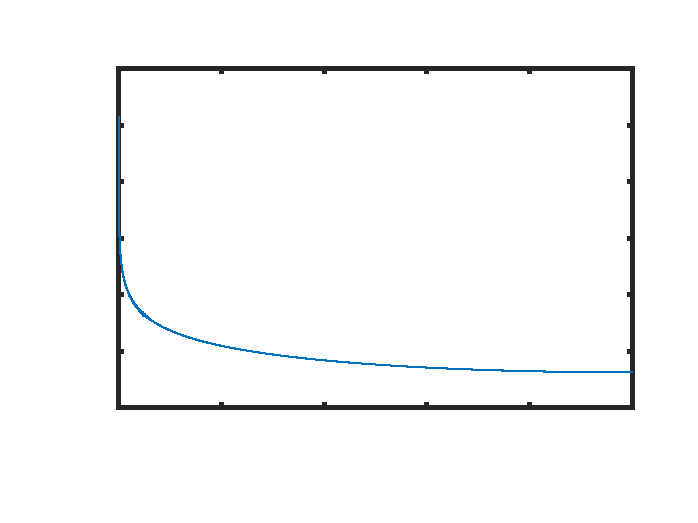
\includegraphics[scale=1]{DoubleKapitzaFourierTheta1-inc}
\end{picture}%
\begin{picture}(335,251)(0,0)
\fontsize{20}{0}\selectfont\put(56.981,40.4535){\makebox(0,0)[t]{\textcolor[rgb]{0.15,0.15,0.15}{{0}}}}
\fontsize{20}{0}\selectfont\put(106.291,40.4535){\makebox(0,0)[t]{\textcolor[rgb]{0.15,0.15,0.15}{{0.1}}}}
\fontsize{20}{0}\selectfont\put(155.601,40.4535){\makebox(0,0)[t]{\textcolor[rgb]{0.15,0.15,0.15}{{0.2}}}}
\fontsize{20}{0}\selectfont\put(204.911,40.4535){\makebox(0,0)[t]{\textcolor[rgb]{0.15,0.15,0.15}{{0.3}}}}
\fontsize{20}{0}\selectfont\put(254.221,40.4535){\makebox(0,0)[t]{\textcolor[rgb]{0.15,0.15,0.15}{{0.4}}}}
\fontsize{20}{0}\selectfont\put(303.531,40.4535){\makebox(0,0)[t]{\textcolor[rgb]{0.15,0.15,0.15}{{0.5}}}}
\fontsize{20}{0}\selectfont\put(46.9992,55.4153){\makebox(0,0)[r]{\textcolor[rgb]{0.15,0.15,0.15}{{10}}}}
\fontsize{20}{0}\selectfont\put(46.9992,82.5127){\makebox(0,0)[r]{\textcolor[rgb]{0.15,0.15,0.15}{{15}}}}
\fontsize{20}{0}\selectfont\put(46.9992,109.61){\makebox(0,0)[r]{\textcolor[rgb]{0.15,0.15,0.15}{{20}}}}
\fontsize{20}{0}\selectfont\put(46.9992,136.708){\makebox(0,0)[r]{\textcolor[rgb]{0.15,0.15,0.15}{{25}}}}
\fontsize{20}{0}\selectfont\put(46.9992,163.805){\makebox(0,0)[r]{\textcolor[rgb]{0.15,0.15,0.15}{{30}}}}
\fontsize{20}{0}\selectfont\put(46.9992,190.903){\makebox(0,0)[r]{\textcolor[rgb]{0.15,0.15,0.15}{{35}}}}
\fontsize{20}{0}\selectfont\put(46.9992,218){\makebox(0,0)[r]{\textcolor[rgb]{0.15,0.15,0.15}{{40}}}}
\fontsize{22}{0}\selectfont\put(180.256,21.4535){\makebox(0,0)[t]{\textcolor[rgb]{0.15,0.15,0.15}{{Frequency}}}}
\fontsize{22}{0}\selectfont\put(21.9992,136.708){\rotatebox{90}{\makebox(0,0)[b]{\textcolor[rgb]{0.15,0.15,0.15}{{log(Power Spectra)}}}}}
\fontsize{22}{0}\selectfont\put(180.256,228){\makebox(0,0)[b]{\textcolor[rgb]{0,0,0}{{Power Spectra of $\theta_1$}}}}
\end{picture}
\end{document}
